%%%%%%%%%%%%%%%%%%%%%%%%%%%%%%%%%%%%%%%%%%%%%%
% Head matter - can we try to be consistent on
% included packages
\ifdefined\beamerclass
\else
    \def\beamerclass{beamer}
\fi
\documentclass[\beamerclass]{beamer}

\usepackage{pgfpages}
\usepackage{pgfplots}
\mode<handout>{
  % \setbeamercolor{background canvas}{bg=black!20}
  \pgfpagesuselayout{2 on 1}[a4paper,border shrink=5mm]
}

%\documentclass{beamer}
\mode<presentation>
{\usetheme{default}
 \usecolortheme{default}
 \usefonttheme{default}
 \setbeamertemplate{navigation symbols}{}
 \setbeamertemplate{footline}[frame number]
% \setbeamertemplate{caption}[numbered]
 }
\usepackage[english]{babel}
\usepackage{algorithm}
\usepackage[noend]{algpseudocode}
\usepackage[utf8x]{inputenc}
\usepackage{graphicx}
\usepackage{hyperref}
%\graphicspath{{./images/}}
\usepackage{tikz}
\usetikzlibrary{shapes.geometric, arrows,chains}
\usepackage{booktabs,makecell,multirow,tabularx}
\usepackage{verbatim}
\renewcommand{\arraystretch}{1.2}
\renewcommand\theadfont{\normalfont\bfseries}
\usepackage{array}
\usepackage{listings}
\lstset{language=Java, showstringspaces=false}
\usepackage[normalem]{ulem}
\usepackage{bm}
\def\layersep{2.5cm}

\usepackage{xcolor}
%\usepackage{subfig}
\setbeamertemplate{caption}{\insertcaption}
\usepackage[caption=false]{subfig}
\usepackage{hyperref}
\usepackage{verbatim}
%\setbeamertemplate{caption}[numbered]%\numberwithin{figure}{section}
% Define block styles

\usetheme{Copenhagen}
\hypersetup{pdfstartview={Fit}}
\lstset{basicstyle=\small\ttfamily,breaklines=true}

\usepackage{xmpmulti}

\tikzstyle{decision} = [diamond, draw, fill=blue!20, 
    text width=4.5em, text badly centered, node distance=3cm, inner sep=0pt]
\tikzstyle{block} = [rectangle, draw, fill=blue!20, 
    text width=3em, text centered, rounded corners, minimum height=3em]
\tikzstyle{line} = [draw, -latex']
\tikzstyle{cloud} = [draw, ellipse, fill=red!20, node distance=3cm,
    minimum height=2em]
\tikzset{
  startstop/.style={
    rectangle, 
    rounded corners,
    minimum width=3cm, 
    minimum height=1cm,
    align=center, 
    draw=black, 
    fill=red!30
    },
  process/.style={
    rectangle, 
    minimum width=3cm, 
    minimum height=1cm, 
    align=center, 
    draw=black, 
    fill=blue!30
    },
  decision/.style={
    rectangle, 
    minimum width=3cm, 
    minimum height=1cm, align=center, 
    draw=black, 
    fill=green!30
    },
  arrow/.style={thick,->,>=stealth},
  dec/.style={
    ellipse, 
    align=center, 
    draw=black, 
    fill=green!30
    },
}
\tikzstyle{arrow} = [thick,->,>=stealth]

\tikzset{onslide/.code args={<#1>#2}{%
  \only<#1>{\pgfkeysalso{#2}} % \pgfkeysalso doesn't change the path
}}

\makeatletter
\newenvironment<>{btHighlight}[1][]
{\begin{onlyenv}#2\begingroup\tikzset{bt@Highlight@par/.style={#1}}\begin{lrbox}{\@tempboxa}}
{\end{lrbox}\bt@HL@box[bt@Highlight@par]{\@tempboxa}\endgroup\end{onlyenv}}

\newcommand<>\btHL[1][]{%
  \only#2{\begin{btHighlight}[#1]\bgroup\aftergroup\bt@HL@endenv}%
}
\def\bt@HL@endenv{%
  \end{btHighlight}%   
  \egroup
}
\newcommand{\bt@HL@box}[2][]{%
  \tikz[#1]{%
    \pgfpathrectangle{\pgfpoint{1pt}{0pt}}{\pgfpoint{\wd #2}{\ht #2}}%
    \pgfusepath{use as bounding box}%
    \node[anchor=base west, fill=orange!30,outer sep=0pt,inner xsep=1pt, inner ysep=0pt, rounded corners=3pt, minimum height=\ht\strutbox+1pt,#1]{\raisebox{1pt}{\strut}\strut\usebox{#2}};
  }%
}
\makeatother

\definecolor{darkblue}{RGB}{37,55,97}
\definecolor{mellowyellow}{RGB}{247,206,70}
\definecolor{almostwhite}{RGB}{254,255,255}
\definecolor{merrygreen}{RGB}{79,173,91}
\definecolor{funkyorange}{RGB}{240,154,56}

\addtobeamertemplate{footnote}{\hskip -2em}{}
\newcommand\blfootnote[1]{%
  \begingroup
  \renewcommand\thefootnote{}\footnote{#1}%
  \addtocounter{footnote}{-1}%
  \endgroup
}

\DeclareMathOperator{\softmax}{softmax}
\DeclareMathOperator{\softplus}{softplus}
\DeclareMathOperator{\ReLU}{ReLU}
\DeclareMathOperator{\argmax}{arg\,max}
\DeclareMathOperator{\abs}{abs}
\DeclareMathOperator{\huber}{huber}

%%%%%%%%%%%%%%%%%%%%%%%%%%%%%%%%%%%%%%%%%%%%%%
% Formatting for title page
\title[Relaxation]{Differentiable Relaxations and Reparameterisations}
\author{Jonathon Hare}
\institute[]
{
  Vision, Learning and Control\\
  University of Southampton 
}
\date{}
\subject{Computer Science}
\useoutertheme{infolines}
\setbeamertemplate{headline}{} %remove headline
\setbeamertemplate{navigation symbols}{} %remove navigation symbols
%%%%%%%%%%%%%%%%%%%%%%%%%%%%%%%%%%%%%%%%%%%%%%

\begin{document}

\begin{frame}[plain]
        \begin{tikzpicture}[overlay, remember picture, shift={(current page.south west)},font={\fontfamily{Montserrat-TOsF}\selectfont}]
        \fill [merrygreen,text=almostwhite] (0,0) rectangle (\paperwidth, \paperheight);
        \draw (5.5,7) node [align=left,text=almostwhite] {\Huge 
        \begin{tabular}{l} 
        \textbf{Differentiate}\\
        \textbf{Almost} \\
        \textbf{Everywhere} 
        \end{tabular}};
        \draw (11,1) node [align=left,text=almostwhite] {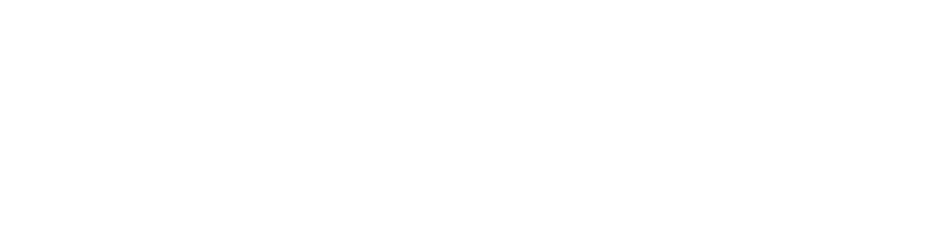
\includegraphics[scale=0.15]{../vlc.png}};
        \end{tikzpicture}
\end{frame}

\begin{frame}
  \titlepage
\end{frame}

%-------------------------------------------------------------%

\begin{frame}
\frametitle{What are differentiable relaxations and reparameterisations?}
 
\begin{itemize}
  \item<+-> We've seen that we can build arbitrary computational graphs from a variety of building blocks
  \item<+-> But, those blocks need to be differentiable to work in our optimisation framework
  \begin{itemize}
    \item More specifically they need to be continuous and \emph{differentiable almost everywhere}.
  \end{itemize}
  \item<+-> That limits what we can do... Can we work around that?
  \begin{itemize}
    \item Relaxations --- make continuous (and potentially differentiable everywhere) approximations.
    \item Reparameterisations --- rewrite functions to factor out stochastic variables from the parameters.
  \end{itemize}
\end{itemize}


\end{frame}

%-------------------------------------------------------------%

\begin{frame}
\frametitle{Aside: continuity and differentiable almost everywhere}

\begin{itemize}
  \item<+-> Consider the $\ReLU$ function $f(x) = max(0,x)$
  \begin{itemize}
    \item<+-> $\ReLU$ is \emph{continuous}
    \begin{itemize}
      \item it does not have any abrupt changes in value
      \item small changes in $x$ result in small changes to $f(x)$ everywhere in the domain of $x$
    \end{itemize}
    \item<+-> $\ReLU$ is \emph{differentiable almost everywhere}
    \begin{itemize}
      \item No gradient at $x=0$; only \emph{left} and \emph{right} gradients at that point
      \item There are \emph{subgradients} at $x=0$; implementations usually just arbitrarily pick $f'(0)=0$
    \end{itemize}
  \end{itemize}
  \item<+-> Functions that are differentiable almost everywhere or have subgradients tend to be compatible with gradient descent methods
  \begin{itemize}
    \item We expect that the loss landscape is different for each batch \& that we'll never actually reach a minima, and we only need to \emph{mostly} take steps in the right direction.
  \end{itemize}
\end{itemize}
\end{frame}

%-------------------------------------------------------------%

\begin{frame}
\frametitle{Relaxing $\ReLU$}

\begin{columns}
\begin{column}{0.6\textwidth}
   \begin{itemize}
     \item<+-> Softplus ($\softplus(x) = \ln(1+e^x)$) is a relaxation of $\ReLU$ that is \emph{differentiable everywhere}.
     \item<+-> Its derivative is the Sigmoid function
     \item<+-> Not widely used; counter-intuitively, even though it neither saturates completely and is differentiable everywhere, empirically it has been shown that $\ReLU$ works better.
   \end{itemize}
\end{column}
\begin{column}{0.4\textwidth}
\begin{tikzpicture}
  \begin{axis}[ 
    % xlabel=$x$,
    % ylabel=$f(x)$,
    height=5cm,
    width=5cm,
    grid=major,
    axis equal,
  ] 
    \addplot[red] {max(0,x)}; 
    \addlegendentry{$\ReLU$}

    \addplot[blue] {ln(1 + exp(x))}; 
    \addlegendentry{Softplus}
  \end{axis}
\end{tikzpicture}
\end{column}
\end{columns}

\end{frame}

%-------------------------------------------------------------%

\begin{frame}
\frametitle{Interpretations of $\softmax$}

\begin{itemize}
  \item<+-> Up until now we've really considered $\softmax$ as a generalisation of sigmoid (which represents a probability distribution over a binary variable) to many output categories.
  \begin{itemize}
    \item $\softmax$ transforms a vector of logits into a probability distribution over categories.
  \end{itemize}
\item<+-> As you might guess from the name, $\softmax$ is a relaxation...
\begin{itemize}
  \item<+-> but not of the $\max$ function like the name would suggest!
  \item<+-> $\softmax$ can be viewed as a continuous and differentiable relaxation of the $\argmax$ function with one-hot output encoding.
  \item<+-> The $\argmax$ function is not continuous or differentiable; $\softmax$ provides an approximation:

  \begin{tabular}{crlllll}
  $\bm x = $ & [ & 1.1 & 4.0 & -0.1 & 2.3 & ] \\
  $\argmax(\bm x) = $ & [ & 0 & 1 & 0 & 0 & ] \\
  $\softmax(\bm x) = $ &  [ & 0.044 & 0.797 & 0.013 & 0.146 & ] \\
  \end{tabular}
\end{itemize}
\end{itemize}

\end{frame}

\begin{frame}
\frametitle{The Softmax function with temperature}
Consider what happens if you were to divide the input logits to a $\softmax$ by a scalar temperature parameter $T$.

\begin{center}
$\softmax(\bm x / T)_i = \frac{e^{x_i / T}}{\sum_{j=1}^K e^{x_j / T}} \;\;\;\;\;\;\; \forall i = 1, 2, \dots, K$  
\end{center}

\begin{figure}
\centering
\begin{tikzpicture}
  \begin{axis}[
    % xlabel=Cost,
    % ylabel=Error,
    ybar, 
    xtick=data,
    enlargelimits=0.15,
    bar width=9pt,
    height=7cm,
    width=10cm,]
  \addplot coordinates {
    (0,0.2404)
    (1,0.2779)
    (2,0.2264)
    (3,0.2553)
  };
  \addplot coordinates {
    (0,0.2064)
    (1,0.3687)
    (2,0.1624)
    (3,0.2624)
  };
  \addplot coordinates {
    (0,0.0439)
    (1,0.7973)
    (2,0.0132)
    (3,0.1456)
  };
  \addplot coordinates {
    (0,2.9204e-03)
    (1,9.6462e-01)
    (2,2.6494e-04)
    (3,3.2193e-02)
  };
  \legend{$T=20.0$, $T=5.0$, $T=1.0$, $T=0.5$}
  \end{axis}
\end{tikzpicture}  
\end{figure}


\end{frame}


\begin{frame}
\frametitle{$\argmax$ --- $\softmax$ with temperature}

\begin{tabular}{crlllll}
$\bm x = $ & [ & 1.1 & 4.0 & -0.1 & 2.3 & ] \\
$\softmax(\bm x/1.0) = $ & [ & 0.044 & 0.797 & 0.013 & 0.146 & ]\\
$\softmax(\bm x/0.8) = $ & [ & 0.023 & 0.868 & 0.005 & 0.104 & ]\\
$\softmax(\bm x/0.6) = $ & [ & 0.008 & 0.937 & 0.001 & 0.055 & ]\\
$\softmax(\bm x/0.4) = $ & [ & 6.997e-04 &  9.852e-01 & 3.484e-05 & 1.405e-02 & ] \\
$\softmax(\bm x/0.2) = $ & [ & 5.042e-07 &  9.998e-01 & 1.250e-09 & 2.034e-04 & ] \\
\end{tabular}

\end{frame}

\begin{frame}
\frametitle{$\argmax$ --- scalar approximation}

\begin{itemize}
  \item<+-> What if you want to get a scalar approximation to the index of the $\argmax$ rather than a probability distribution approximating the one-hot form?
  \begin{itemize}
    \item Caveat: we are not actually going get a guaranteed integer representation as that would be non-differentiable; we'll have to live with a float that is an approximation\footnote{for now --- we'll address this in a few slides time!}.
  \end{itemize}
  \item<+-> First, consider how to convert a one-hot vector to index representation in a differentiable manner: $[0,0,1,0] \to 2$
  \begin{itemize}
    \item Just dot product with a vector of indices: $[0,1,2,3]$
  \end{itemize}
  \item<+-> The same process can be applied to the $\softmax$ distribution
  \begin{itemize}
    \item As temperature $T \to 0$, $\softmax(\bm x / T) \cdot [0, 1, \dots, N] \to \argmax(\bm x)$ for $\bm x \in \mathbb{R}^N$.
  \end{itemize}
\end{itemize}
\end{frame}

\begin{frame}
\frametitle{$\argmax$ --- scalar approximation}

\centering
\begin{align*}
\bm x &= [ \begin{array}{cccc}1.1 & 4.0 & -0.1 & 2.3\end{array}]^\top \\
\bm i &= [ \begin{array}{cccc}0.0 & 1.0 & 2.0 & 3.0\end{array}]^\top \\
\softmax(\bm x/1.0)^\top \bm i &= 1.2606 \\
\softmax(\bm x/0.8)^\top \bm i &= 1.1894 \\
\softmax(\bm x/0.6)^\top \bm i &= 1.1037 \\
\softmax(\bm x/0.4)^\top \bm i &= 1.0274 \\
\softmax(\bm x/0.2)^\top \bm i &= 1.0004 \\
\end{align*}
\end{frame}


\begin{frame}
\frametitle{max}

\begin{itemize}
  \item<+-> A similar trick applies to finding the maximum value of a vector:
  \begin{itemize}
    \item<+-> Use $\softmax(\bm x)$ as an approximate one-hot $\argmax$, and dot product with the vector $\bm x$.
    \item<+-> As temperature $T \to 0$, $\softmax(\bm x / T)^\top \bm x \to \max(\bm x)$.
  \end{itemize}
\end{itemize}

\only<+->{
\centering
\begin{align*}
\bm x &= [ \begin{array}{cccc}1.1 & 4.0 & -0.1 & 2.3\end{array}]^\top \\
\softmax(\bm x/1.0)^\top \bm x &= 3.571 \\
\softmax(\bm x/0.8)^\top \bm x &= 3.736 \\
\softmax(\bm x/0.6)^\top \bm x &= 3.881 \\
\softmax(\bm x/0.4)^\top \bm x &= 3.974 \\
\softmax(\bm x/0.2)^\top \bm x &= 3.999 \\
\end{align*}
}
\end{frame}

%-------------------------------------------------------------%

\begin{frame}
\frametitle{L1 norm}

\begin{columns}
\begin{column}{0.6\textwidth}   
\begin{itemize}
  \item<+-> L1 norm is the sum of absolute values of a vector
  \item<+-> We've seen that an L1 norm regulariser can induce sparsity in a model
  \item<+-> $\abs$ is continuous and differentiable almost everywhere, but...
  \item<+-> unlike ReLU, the gradients left and right of the discontinuity point in equal and opposite directions
  \begin{itemize}
    \item This can cause oscillations that prevent or hamper learning
  \end{itemize}
\end{itemize}
\end{column}
\begin{column}{0.4\textwidth}
\begin{tikzpicture}[
declare function={
    dAbs(\x)= (\x<0) * (-1) + (\x>0) * (1);
  }
]
  \begin{axis}[ 
    % xlabel=$x$,
    % ylabel=$f(x)$,
    height=5cm,
    width=5cm,
    grid=major,
    axis equal,
    samples=1001
  ] 
    \addplot[blue] {abs(x)}; 
    \addlegendentry{$\abs(x)$}

    \addplot[red] {dAbs(x))}; 
    \addlegendentry{$\abs'(x)$}
  \end{axis}
\end{tikzpicture}

\end{column}
\end{columns}
\end{frame}

\begin{frame}
\frametitle{Relaxing the L1 norm}

\begin{columns}
\begin{column}{0.6\textwidth}   
\begin{itemize}
  \item<+-> Huber loss (aka Smooth L1 loss) relaxes L1 by mixing it with L2 near the origin:
  \begin{equation*}
    z_{i} =
        \begin{cases}
        0.5 (x_i - y_i)^2, & \text{if } |x_i - y_i| < 1 \\
        |x_i - y_i| - 0.5, & \text{otherwise }
        \end{cases}
  \end{equation*}

  \item<+-> In both cases gradients reduce in magnitude and switch direction smoothly which can lead to much less oscillation.
\end{itemize}
\end{column}
\begin{column}{0.4\textwidth}
\begin{tikzpicture}[
declare function={
    huber(\x)= (abs(\x)>=1) * (abs(x) - 0.5) + (abs(\x)<1) * (0.5 * x^2);
  },
declare function={
    dhuber(\x)= (\x>=1) * (1) + (abs(\x)<1) * (x) + (\x<=-1) * (-1);
  }
]
  \begin{axis}[ 
    % xlabel=$x$,
    % ylabel=$f(x)$,
    height=5cm,
    width=5cm,
    grid=major,
    axis equal,
    samples=1001
  ] 
    \addplot[blue] {huber(x))}; 
    \addlegendentry{$\huber(x)$}

    \addplot[red] {dhuber(x))}; 
    \addlegendentry{$\huber'(x)$}
  \end{axis}
\end{tikzpicture}

\end{column}
\end{columns}
\end{frame}

%-------------------------------------------------------------%

\begin{frame}
\frametitle{Backpropagation through random operations}

\begin{itemize}
  \item<+-> Up until now all the models we've considered have performed deterministic transformations of input variables $\bm x$.
  \item<+-> What if we want to build a model that performs a stochastic transformation of $\bm x$?
  \item<+-> A simple way to do this is to augment the input $\bm x$ with a random vector $\bm z$ sampled from some distribution 
  \begin{itemize}
    \item<+-> The network would learn a function $f(\bm x, \bm z)$ that is internally deterministic, but appears stochastic to an observer that does not have access to $\bm z$.
    \item<+-> provided that $f$ is continuous and differentiable (almost everywhere) we can perform gradient based optimisation as usual.
  \end{itemize}
\end{itemize}

\end{frame}

\begin{frame}
\frametitle{Differentiable Sampling}

Consider 
\begin{equation*}
  y \sim \mathcal{N}(\mu, \sigma^2) 
\end{equation*}
How can we take derivatives of $y$ with respect to $\mu$ and $\sigma^2$?

\end{frame}

%-------------------------------------------------------------%

\begin{frame}
\frametitle{Differentiable Sampling}

If we rewrite
\begin{equation*}
y = \mu + \sigma z \; \mathrm{where}\; z = \mathcal{N}(0,1)
\end{equation*}
Then it is clear that $y$ is a function of a deterministic operation with variables $\mu$ and $\sigma$ with an (extra) input $z$. 
\begin{itemize}
  \item<+-> Crucially the extra input is an r.v. whose distribution is not a function of any variables whose derivatives we wish to calculate.
  \item<+-> The derivatives $dy/d\mu$ and $dy/d\sigma$ tell us how an infinitesimal change in $\mu$ or $\sigma$ would change $y$ if we could repeat the sampling operation with the \emph{same} value of $z$
\end{itemize}
\end{frame}

%-------------------------------------------------------------%

\begin{frame}
\frametitle{The reparameterisation trick}

\begin{itemize}
  \item<+-> The `trick' of factoring out the source of randomness into an extra input $z$ is often called the \textbf{reparameterisation trick}.
  \item<+-> It doesn't just apply to the Gaussian distribution!
  \begin{itemize}
    \item<+->More generally we can express any probability distribution $p(\mathrm{y}; \bm\theta)$ or $p(\mathrm{y} | \bm x; \bm\theta)$ as $p(\mathrm{y}; \bm\omega)$ where $\bm\omega$ contains the parameters $\bm\theta$ and if applicable inputs $\bm x$.
      \item<+-> A sample $\bm y \sim p(\mathrm{y}; \bm\omega)$ can be rewritten as $\bm y=f(\bm z, \bm\omega)$ where $\bm z$ is a source of randomness.
      \item<+-> We can thus compute derivatives $\partial \bm y/\partial \bm\omega$ and use gradient based optimisation as long as
      \begin{itemize}
        \item $f$ is continuous and differentiable almost everywhere
        \item $\bm\omega$ is not a function of $\bm z$
        \item and $\bm z$ is not a function of $\bm\omega$
      \end{itemize}
    \end{itemize}
\end{itemize}

\end{frame}

%-------------------------------------------------------------%

\begin{frame}
\frametitle{Backpropagation through discrete stochastic operations}

\begin{itemize}
  \item<+-> Consider a stochastic model $\bm y = f(\bm z, \bm \omega)$ where the outputs are \textbf{discrete}. 
  \begin{itemize}
    \item<+-> This implies $f$ must be a step function.
    \item<+-> Derivatives of a step function at the step are undefined.
    \item<+-> Derivatives are zero almost everywhere. 
    \item<+-> If we have a loss $\mathcal{L}(\bm y)$ the gradients don't give us any information on how to update the parameters $\bm\theta$ to minimise the loss
  \end{itemize}
  \item<+-> Potential solutions:
  \begin{itemize}
    \item Policy Gradient Methods (e.g. the REINFORCE algorithm)
    \item A relaxation and another `trick': Gumbel Softmax and the Straight-through operator
  \end{itemize}
\end{itemize}

\end{frame}

%-------------------------------------------------------------%

\begin{frame}
\frametitle{REINFORCE: REward Increment = nonnegative Factor $\times$ Offset Reinforcement $\times$ Characteristic Eligibility}

\begin{itemize}
  \item<+-> $\mathcal{L}(f(\bm z, \bm\omega))$ has useless derivatives
  \item<+-> But the expected loss $\mathbb{E}_{\bm z \sim p(\mathbf{z})} \mathcal{L}(f(\bm z, \bm \omega))$is often smooth and continuous.
  \begin{itemize}
    \item This is not tractable with high dimensional $\bm y = f(\bm z, \bm \omega)$.
    \item But, it can be estimated without bias using an Monte Carlo average.
  \end{itemize}
  \item<+-> REINFORCE is a family of algorithms that utilise this idea.
\end{itemize}

\end{frame}

%-------------------------------------------------------------%

\begin{frame}
\frametitle{REINFORCE: REward Increment = nonnegative Factor $\times$ Offset Reinforcement $\times$ Characteristic Eligibility}

The simplest form of REINFORCE is easy to derive by differentiating the expected loss:
\footnotesize
\begin{align}
\mathbb{E}_{\bm z}[\mathcal{L}(\bm y)] &= \sum_{\bm y} \mathcal{L}(\bm y)p(\bm y)\\
\frac{\partial \mathbb{E}[\mathcal{L}(\bm y)]}{\partial \bm\omega} &= \sum_{\bm y} \mathcal{L}(\bm y) \frac{\partial p(\bm y)}{\partial \bm\omega}\\
&= \sum_{\bm y} \mathcal{L}(\bm y) p(\bm y) \frac{\partial \log p(\bm y)}{\partial \bm\omega}\\
&\approx \frac{1}{m} \sum_{\bm y^{(i)} \sim p(\mathbf{y}), i=1}^{m} \mathcal{L}(\bm y^{(i)}) \frac{\partial \log p(\bm y^{(i)})}{\partial \bm\omega}
\end{align}
\normalsize

\begin{itemize}
  \item<+-> This gives us an unbiased MC estimator of the gradient.
  \item<+-> Unfortunately this is a very high variance estimator, so it would require many samples of $y$ to be drawn to obtain a good estimate
  \begin{itemize}
    \item<+-> or equivalently, if only one sample were drawn, SGD would converge very slowly and \textbf{require} a small learning rate.
  \end{itemize}
\end{itemize}

\end{frame}


%-------------------------------------------------------------%

\begin{frame}
\frametitle{Sampling from a categorical distribution: Gumbel Softmax}

The generation of a discrete token, $t$, from a vocabulary of $K$ tokens is achieved by sampling a categorical distribution 
\begin{equation*}
t \sim \operatorname{Cat}(p_1, \dots, p_K)\,; \,\sum_i p_i=1.
\end{equation*} \pause
Generating the probabilities $p_1, \dots, p_K$ directly from a neural network has potential numerical problems; it's much easier to generate logits, $x_1, \dots, x_K$. \pause
\\[0.5em]
The gumbel-softmax reparameterisation allows us to sample directly using the logits: 
\begin{equation*}
t = \underset{ i \in \{1,\cdots,K\} }{\operatorname{argmax}} x_i + z_i
\end{equation*}
where $z_1, \dots z_K$ are i.i.d Gumbel(0,1) variates  which can be computed from Uniform variates through $-\log(-\log(\mathcal{U}(0,1)))$.

\end{frame}

\begin{frame}
\frametitle{Differentiable Sampling: Straight-Through Gumbel Softmax}
Ok, but how does that help? $\operatorname{argmax}$ isn't differentiable! \pause
\\[0.5em]
...but we've already seen that we can relax $\argmax$ using
\begin{equation*}
  \operatorname{softargmax}(\bm y) = \sum_i \frac{e^{y_i/T}}{\sum_j e^{y_j/T}} i
\end{equation*}
where $T$ is the temperature parameter.
\end{frame}

\begin{frame}
\frametitle{Differentiable Sampling: Straight-Through Gumbel Softmax}
But... this clearly gives us a result that will be non-integer; we cannot round or clip because it would be non-differentiable. \pause
\\[0.5em]
The Straight-Through operator allows us to take the result of a true $\operatorname{argmax}$ that has the gradient of the $\operatorname{softargmax}$:
\begin{equation*}
  \operatorname{STargmax}(\bm{y}) = \operatorname{softargmax}(\bm{y}) + \operatorname{stopgradient}(\operatorname{argmax}(\bm{y}) - \operatorname{softargmax}(\bm{y})) 
\end{equation*}
where $\operatorname{stopgradient}$ is defined such that $\operatorname{stopgradient}(\bm{a}) = \bm{a}$ and $\nabla \operatorname{stopgradient}(\bm{a}) = 0$.
\pause
\begin{block}{Straight-Through Gumbel Softmax}
Combine the gumbel softmax trick with the $\operatorname{STargmax}$ to give you discrete samples, with a usable gradient\footnote{The ST operator is biased but low variance; in practice it works very well and is better than the high-variance unbiased estimates you could get through REINFORCE.}.
\end{block}

\end{frame}

\begin{frame}
\frametitle{Summary}

\begin{itemize}
  \item Differentiable programming works with functions that are continuous and differentiable almost everywhere.
  \item Some non-continuous functions can be relaxed to make them more amenable to gradient based optimisation by making continuous approximations.
  \item Some continuous functions with discontinuous gradients can be relaxed to make optimisation more stable.
  \item Reparameterisations can allow us to differentiate through random operations such as sampling
  \item We can even make networks output/utilise discrete variables by combining relaxations and reparameterisations.
\end{itemize}

\end{frame}
\end{document}